% how cryptic is cryptic diversity?
% paper describing the motivation, methods and results of the turtle
% subspecies identification project.
% journal submission order:
%   Systematic Biology (no limit)
%   American Naturalist (21 pages)
%   Journal of Evolutionary Biology

\documentclass[12pt]{article}\usepackage{graphicx, color}
%% maxwidth is the original width if it is less than linewidth
%% otherwise use linewidth (to make sure the graphics do not exceed the margin)
\makeatletter
\def\maxwidth{ %
  \ifdim\Gin@nat@width>\linewidth
    \linewidth
  \else
    \Gin@nat@width
  \fi
}
\makeatother

\definecolor{fgcolor}{rgb}{0.2, 0.2, 0.2}
\newcommand{\hlnumber}[1]{\textcolor[rgb]{0,0,0}{#1}}%
\newcommand{\hlfunctioncall}[1]{\textcolor[rgb]{0.501960784313725,0,0.329411764705882}{\textbf{#1}}}%
\newcommand{\hlstring}[1]{\textcolor[rgb]{0.6,0.6,1}{#1}}%
\newcommand{\hlkeyword}[1]{\textcolor[rgb]{0,0,0}{\textbf{#1}}}%
\newcommand{\hlargument}[1]{\textcolor[rgb]{0.690196078431373,0.250980392156863,0.0196078431372549}{#1}}%
\newcommand{\hlcomment}[1]{\textcolor[rgb]{0.180392156862745,0.6,0.341176470588235}{#1}}%
\newcommand{\hlroxygencomment}[1]{\textcolor[rgb]{0.43921568627451,0.47843137254902,0.701960784313725}{#1}}%
\newcommand{\hlformalargs}[1]{\textcolor[rgb]{0.690196078431373,0.250980392156863,0.0196078431372549}{#1}}%
\newcommand{\hleqformalargs}[1]{\textcolor[rgb]{0.690196078431373,0.250980392156863,0.0196078431372549}{#1}}%
\newcommand{\hlassignement}[1]{\textcolor[rgb]{0,0,0}{\textbf{#1}}}%
\newcommand{\hlpackage}[1]{\textcolor[rgb]{0.588235294117647,0.709803921568627,0.145098039215686}{#1}}%
\newcommand{\hlslot}[1]{\textit{#1}}%
\newcommand{\hlsymbol}[1]{\textcolor[rgb]{0,0,0}{#1}}%
\newcommand{\hlprompt}[1]{\textcolor[rgb]{0.2,0.2,0.2}{#1}}%

\usepackage{framed}
\makeatletter
\newenvironment{kframe}{%
 \def\at@end@of@kframe{}%
 \ifinner\ifhmode%
  \def\at@end@of@kframe{\end{minipage}}%
  \begin{minipage}{\columnwidth}%
 \fi\fi%
 \def\FrameCommand##1{\hskip\@totalleftmargin \hskip-\fboxsep
 \colorbox{shadecolor}{##1}\hskip-\fboxsep
     % There is no \\@totalrightmargin, so:
     \hskip-\linewidth \hskip-\@totalleftmargin \hskip\columnwidth}%
 \MakeFramed {\advance\hsize-\width
   \@totalleftmargin\z@ \linewidth\hsize
   \@setminipage}}%
 {\par\unskip\endMakeFramed%
 \at@end@of@kframe}
\makeatother

\definecolor{shadecolor}{rgb}{.97, .97, .97}
\definecolor{messagecolor}{rgb}{0, 0, 0}
\definecolor{warningcolor}{rgb}{1, 0, 1}
\definecolor{errorcolor}{rgb}{1, 0, 0}
\newenvironment{knitrout}{}{} % an empty environment to be redefined in TeX

\usepackage{alltt}
\usepackage{amsmath, amsthm}
\usepackage{graphicx, microtype, hyperref, authblk}
\usepackage{rotating, longtable, caption, subcaption, multirow}
\usepackage[sort&compress]{natbib}
%\usepackage{fullpage}

% for american naturalist
\usepackage{lineno}

\frenchspacing

% bring in various code necessities
% all the figures are made externally, so this would just be for numerics



\title{How cryptic is cryptic diversity? Machine learning approaches to plastral variation in \textit{Emys marmorata}.}
\author[1]{Peter D Smits \thanks{psmits@uchicago.edu}}
\author[2]{Kenneth D Angielczyk \thanks{kangielczyk@fieldmuseum.org}}
\author[3]{James F Parham \thanks{jparham@fullerton.edu}}
\affil[1]{Committee on Evolution Biology, University of Chicago}
\affil[2]{Department of Geology, Field Museum of Natural History}
\affil[3]{Department of Geological Sciences, California State University -- Fullerton}
\IfFileExists{upquote.sty}{\usepackage{upquote}}{}


\begin{document}

\maketitle

\linenumbers
\modulolinenumbers[2]

\begin{abstract}
  % 200 words

\end{abstract}

\section{Introduction}

% cryptic diversity
%   most species are still deliminated solely based on morphology
%   paleo problem
Cryptic diversity is when taxa were only first deliminated via molecular means and were not or cannot deliminated via morphological identification CITATION. The discovery of this previously unknown diversity has
% all the work done on species delimitation strictly from molecular data
%

Here, we address the question of how much of cryptic diversity may be a product of sample size as well as methodology used for classifying taxa based solely on morphology. Specifically, we ask if fine scale variation in morphology can provide corroboration for subspecific assignment, and if it is possible to determine the best classification hypothesis amongst a few.

% past work on automatic taxon identification and older approaches to classifying taxa
% why use machine learning methods
In the analysis of class differences and identification in morphometric analysis, classification methods such as discriminant analysis and canonical variates analysis CITATIONS have been used frequently for understanding how variation in specific morphologies best differentiate classes of taxa. Additionally, there has been work on the application of neural network models in classification schemes of observations especially in the context of automated taxon identification CITATIONS MACLEOD'S BOOK. Here, we used multiple types of machine learning methods, both unsupervised and supervised, in order to understand the best classification scheme of the taxa. Each method provides a series of unique advantages for understanding how to classify taxa, which are discussed below.


% e. marmorata
%   natural history
%     conservation importance (turtles in general, e. marmorata in specific)
In this study, we address the subspecific classification scheme of \textit{Emys marmorata}, or western pond turtle. \textit{E. marmorata} has a distribution from northern Washington State, USA to Baja California, Mexico.
%   morphological hypothesis of subspecies
%   molecular hypothesis
Traditionally, \textit{E. marmorata} was classified into three subgroups: the northern \textit{E. marmorata marmorata}, the southern \textit{E. marmorata palida}, and a central Californian intergrade zone \citep{Seeliger1945}. \textit{E. marmorata marmorata} is differentiated from \textit{E. marmorata palida} by the presence of a pair of triangular inguinal plates and darker neck markings. It should be noted that the triangular inguinal plates can sometimes be present in \textit{E. marmorata palida} though they are considerably smaller.
More recently, \textit{E. marmorata} was divided into four clades based on mitochrondial DNA: a northern clade, a southern clade, and two central Californian clades \citep{Spinks2005,Spinks2010}. Nuclear DNA supports two major clades, one northern and one southern, however \citet{Spinks2010} argue that the four clade classification is of greater conservation utility to use the mitochondrial classification scheme.
There is now known morphological differentiation between these clades.

% central hypothesis/question of study
% statement of goals and approach
In this study, we apply multiple machine learning approaches to estimate the best classification scheme of \textit{E. marmorata} subspecies based on morphological variation in plastral shape. Because of unclear geographic boundaries between subgroups of \textit{E. marmorata}, we compare two hypotheses of morphology-based classification and two hypotheses of molecular-based classification.


\section{Materials and Methods}
\subsection{Specimens}
We collected morphometric data from 524 specimens. Geographic information was recorded from museum collection information. When precise latitude and longitude information was not known for a specimen, it was inferred from whatever locality information was presented. % museum information?

Specimens were given a class assignment was based on geographic information. Because the exact geographic barriers between different class is unknown and fuzzy, two assignments for both morphological and molecular hypotheses of class were used. 

\subsection{Geometric morphometrics}
% landmarks
Following \citet{Angielczyk2011}, 19 landmarks were digitized using TpsDig 2.04 \citep{Rohlf2005}. 17 of these landmarks are at the endpoints or intersection of the keratinous plastral scutes that cover the platron. These landmarks were chosen to maximize the description of plastral variation. 12 of these landmarks are symmetrical across the axis of symmetry and in order to prevent degrees of freedom and other concerns \citep{Klingenberg2007}, these landmarks were reflected across the axis of symmetry and the average position of each symmetrical pair was used. In cases where damage or incompleteness prevented symetric landmarks from being determined, only the single member of the pair was used. Analysis was then conducted on the resulting ``half'' plastra.

% GP superimposition and PCA
``Half'' plastra landmark configurations were superimposed using generalized Procrustes analysis \citep{Dryden1998a} after which, the principal components of shape were calculated. This was done using the \texttt{shapes} package for R \citep{2013, Dryden2013}.


\subsection{Machine learning analyses}
\subsubsection{Unsupervised learning}
% clustering
%   Riemannian shape distance
Because shape space, or configurations after Procrustes superimposition, is a Riemannian manifold \citep{Dryden1998a} the dissimilarity between each landmark configuration was measured as the Riemmanian shape distance or \(\rho\) \citep{Kendall1984a,Dryden1998a} which should vary between 0 and \(\pi / 2\) assuming no reflection invariance.

%   PAM
The dissimilarity matrix of shape was divisivly clustering using partioning around mediods (PAM) which is analogous to \textit{k}-means clustering except that instead of minimizing the sum of squared Euclidean distances between observations and centroids, the sum of squared dissimilarities between observations and mediods is minimized \citep{Kaufman1990}.
%   gap statistic
The optimal number of clusters of shape configurations is unknown being possibly three, four, or some other value. Clustering solutions were estimated for between 1 and 40 clusters. Clustering solutions were compared using the gap statistic, which is a measure of goodness of clustering \citep{Tibshirani2001a}. Standard errors of the gap statistic for each clustering solution were estimated from 500 bootstrap samples.
%  R implementation
PAM clustering and gap statistic calculation was conducted using the \texttt{cluster} package for R \citep{Maechler2013}.

\subsubsection{Supervised learning}
% training testing split
The dataset of 524 plastron landmarks was split into training and testing datasets. The former was used for model fitting (training) and was 75\% of the total dataset, split proportionally per class, while the testing dataset was used to estimate the effectiveness of each classification scheme (i.e. performance in the wild).

% model types
Two types of supervised learning, or classification, models were fit to the PCs of plastral shape: multinomial logistic regression and random forest. These model types were chosen because of various properties of these models which allow for useful interpretations about the strength and structure of the classification. Multinomial logistic regression models were fit using the \texttt{nnet} package for R \citep{Venables2002} while random forest models were fit using the \texttt{randomForest} package for R \citep{Liaw2002}.

%   multinomial logistic regression
Multinomial logistic regression is an extension of logistic regression, where instead of a binary response it is possible to have three or more response classes CITATION. Effectively, this type of model can be viewed as multiple, simultaneous logistic regression models for each class and the final classification of the observation being the most probable of all the sub-model classifications. From the final model the relative risk of a given classification, with reference to a given class, can be calculated from the coefficients of the features, or predictors. This is similar to the log-odds calculated from the coefficients of a logistic regression.

%   random forest
Random forest models are an extension of classification and regression trees (CART) CITATION. Basically, CARTs are built for random subsamples of both the features of the proposed model and observations. This process is repeated many times, 1000 times here, and the final model is chosen as the mode of the parameter estimates from the distribution of CARTs CITATION. In addition to fitting a classification model, this procedure allows for the features to be ranked in order of importance, means that the variables most important for determining a given classification scheme can be estimated. In the context of predicting class from geometric morphometric data, this identifies the PCs that describe the variation that best distinguishes the different classes.
%   R statement


% model training
%   tuning parameters
%     grid search
%       what are the tuning parameters for each model?
%     best AUC ROC
For both types of supervised learning models, tuning parameters were estimated using 10 rounds of 10-fold cross-validation (CV) across a grid search of all tuning parameter combinations. Optimal tuning parameter values were selected based on area under the receiver operating characteristic curve (AUC ROC). Multiclass AUC ROC was estimated using the all-against one strategy derived by \citet{Hand2001} in implemented in PROC PACKGE.

%   model selection
%     AICc
For the multinomial logistic regression models, PCs were added sequentially in order to increase the overall amount of variation in shape included in each model and the final model was that with the lowest AICc \citep{Burnham2002a} AKAIKE AND OTHER CITATION. This procedure was used because the optimal number of PCs to include is unknown, and while including all of the PCs of shape would mean that all of the variability in plastron shape would be used to estimate class, this may cause the model to be over fit and not provide an accurate estimate of unsampled plastral variation. The maximum number of PCs allowed to be used as predictors was 10 because of both the number of parameters estimated per model and the necessary sample size needed to estimate that many parameters accurately.

%     recursive feature selection
Because random forest models are not fit using maximum likelihood, a recursive feature selection algorithm was used to choose the optimal number of PCs to include based on the AUC ROC of the model. PCs were sequentially added as features until the AUC ROC of the model did not increase. Random forest model parameters were estimated from 1000 subtrees. After each PC was added, 10-fold CV was used to estimate the optimal values of the tuning parameters as well as quantify the uncertainty of each model. Like the multinomial logistic regression models, 10 was the maximum number of PCs that could have been included in the model. The recursive feature selection algorithm used here is that implemented in the \texttt{caret} package for R \citep{Kuhn2013}.

% generalization
%   bootstrap resample of AUC ROC
The final selected models were then used to estimate the class assignments of the training dataset. Model performance was measured using AUC ROC. A distribution of AUC ROC values were estimated for each classification scheme using 1000 nonparametric bootstrap resamples of the training dataset.

\section{Results}
\subsection{Geometric morphometrics}

\subsection{Machine learning analyses}
\subsubsection{Unsupervised learning}

% PAM results
Comparison of the gap statistic values for the different PAM solutions indicates that the optimal number of clusters is 1 (Fig. \ref{fig:gap}). The second best clustering solution is two clusters, however there is no geographic structure to this classification scheme SUPPLEMENT?. Our dataset does not include enough or detailed information on the sex of each \textit{E. marmorata} specimen, thus it is not possible to determine if this clustering solution corresponds to sexual dimorphism between the observations. Male Emyidine turtles are known to have a plastral concavity
Increasing the number of clusters does appear to improve the gap statistic enough to merit comparison. 

% figure
%   gap statistic results
\begin{figure}[ht]
  \centering
  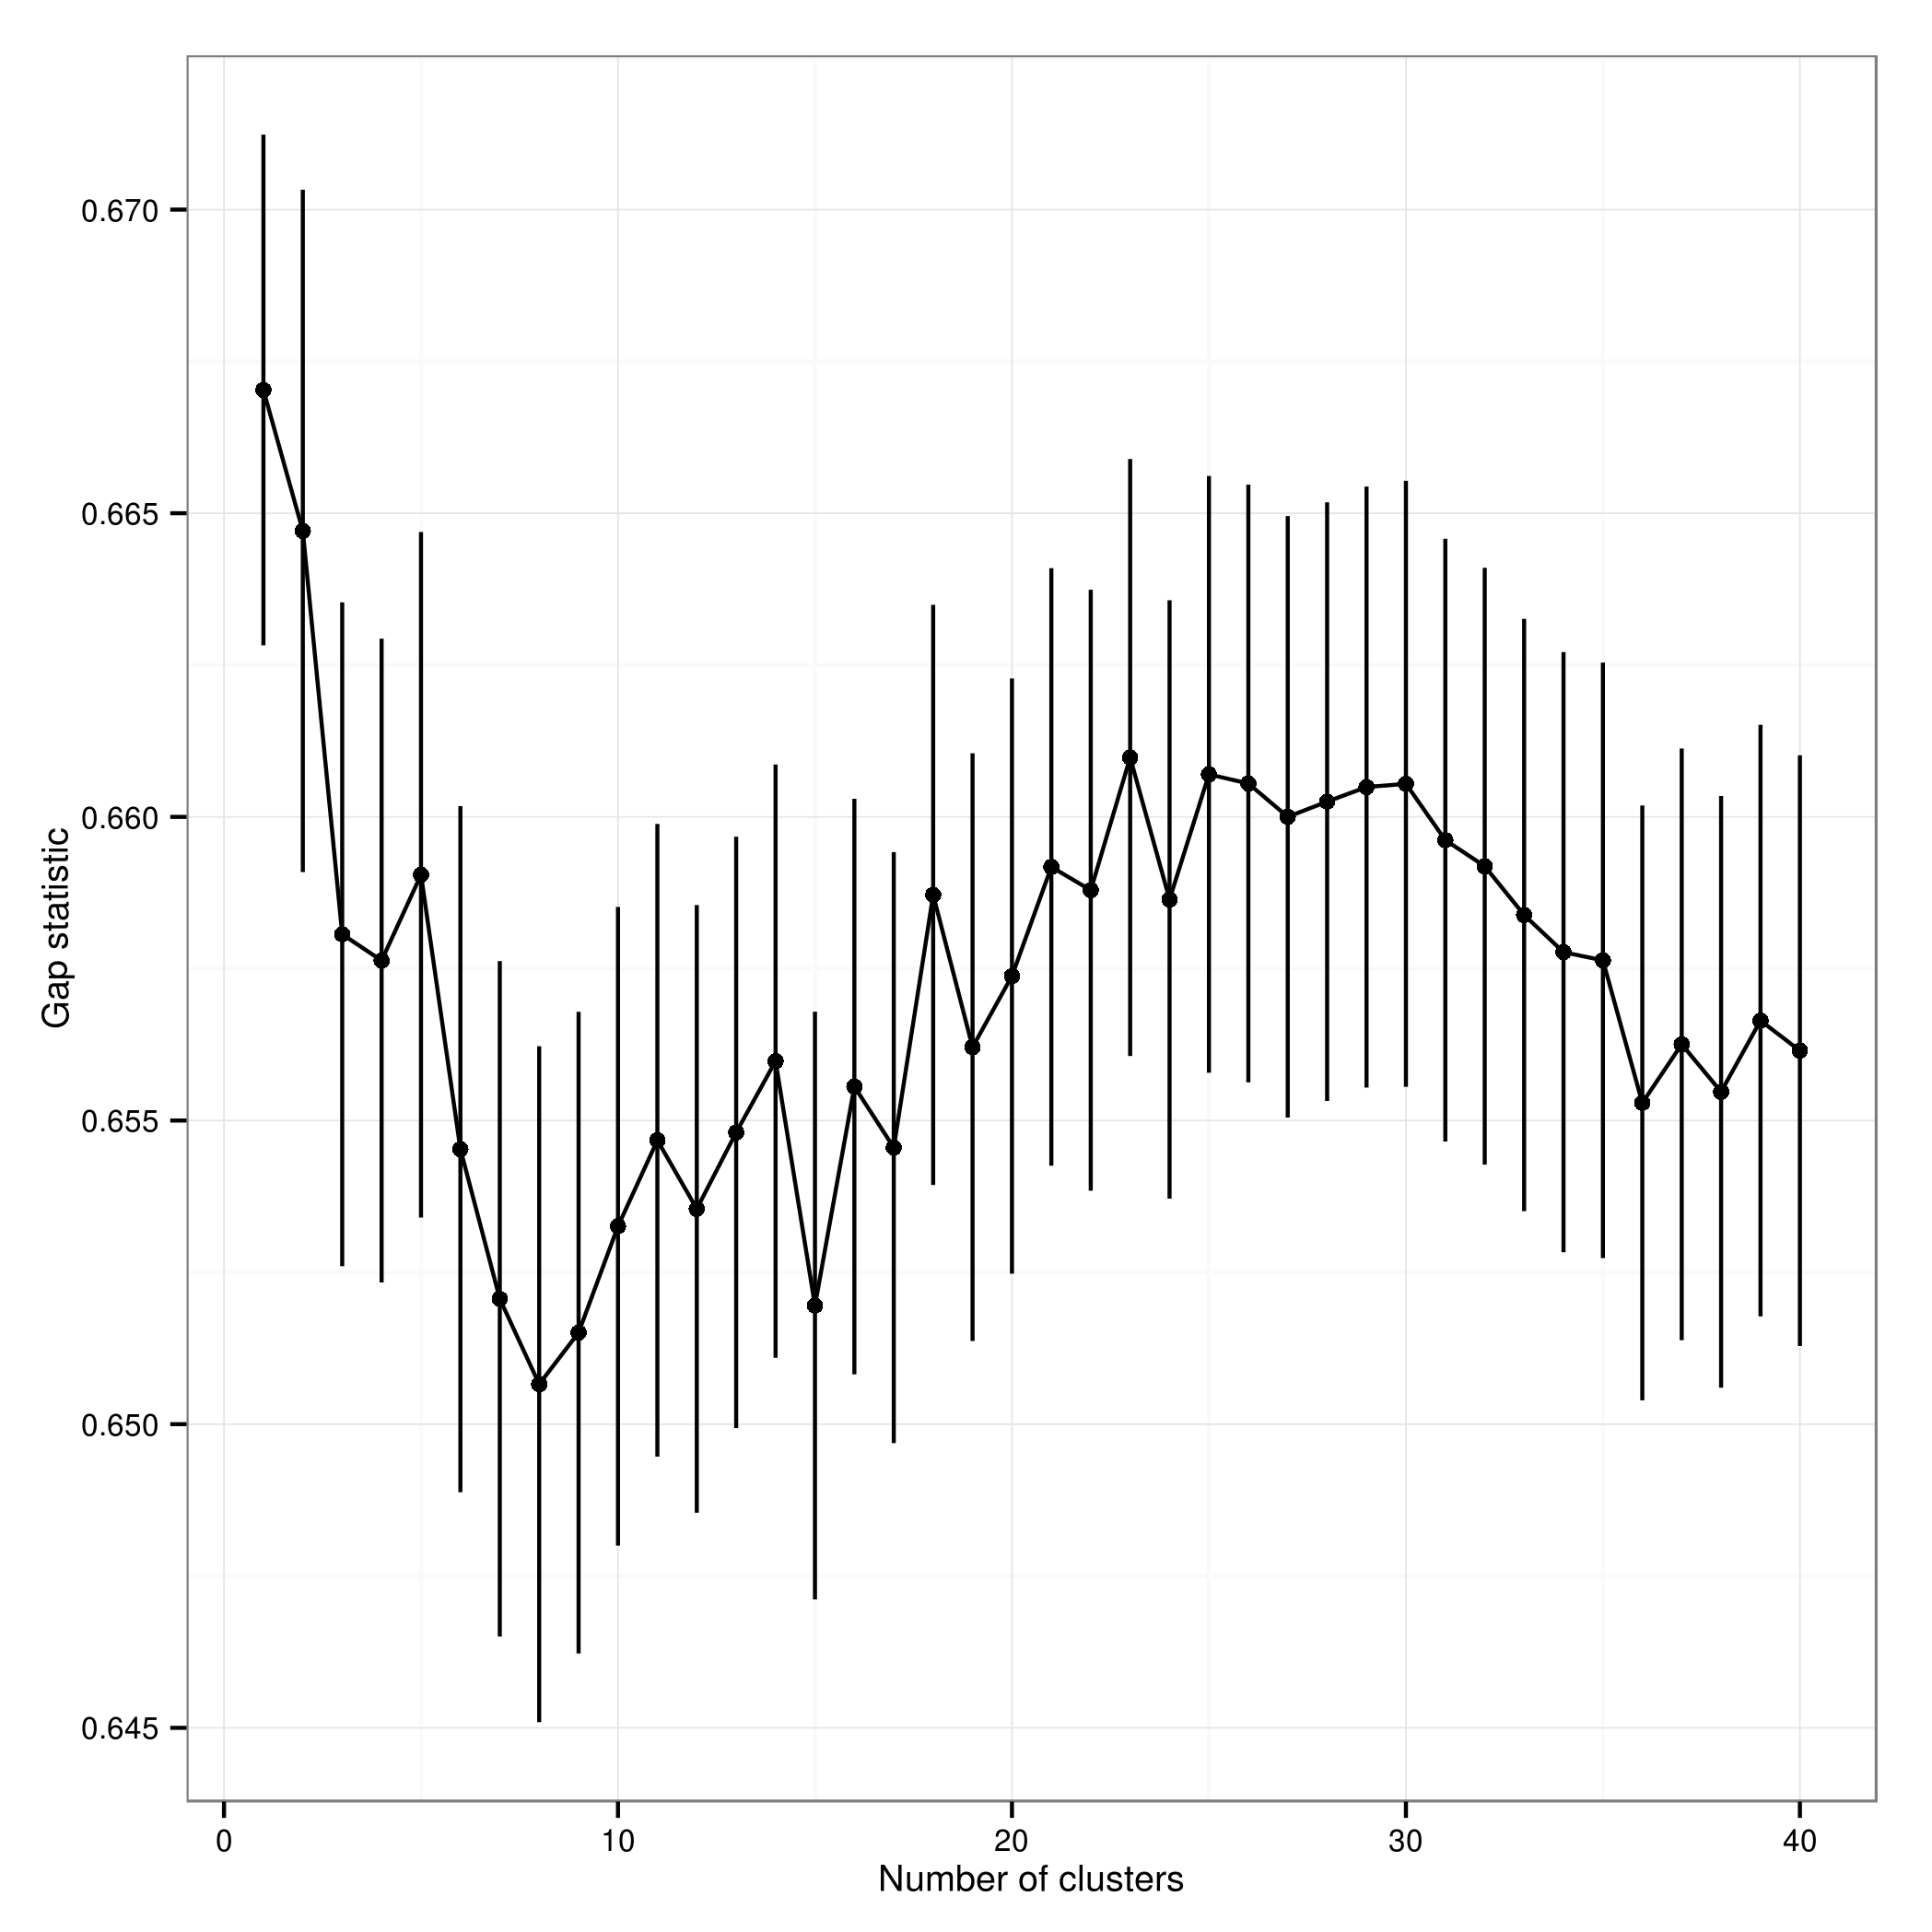
\includegraphics[width = \textwidth]{figure/gap_res}
  \caption{Gap statistic values for PAM clustering results for the \(\rho\) dissimliarity matrix of plastron shape. Error bars are standard errors estimated via 500 bootstrap samples.}
  \label{fig:gap}
\end{figure}

\subsubsection{Supervised learning}
For all classification schemes, the optimal random forest model based on recursive feature selection by maximizing AUC ROC of the model was one with many features (Fig. \ref{fig:roc})
% need to discuss the final models in both cases.
% figure
%   ROC model selection (see talk)
%   generalize densities
%     facet: multinomial, rf (see talk)

\begin{figure}[ht]
  \centering
  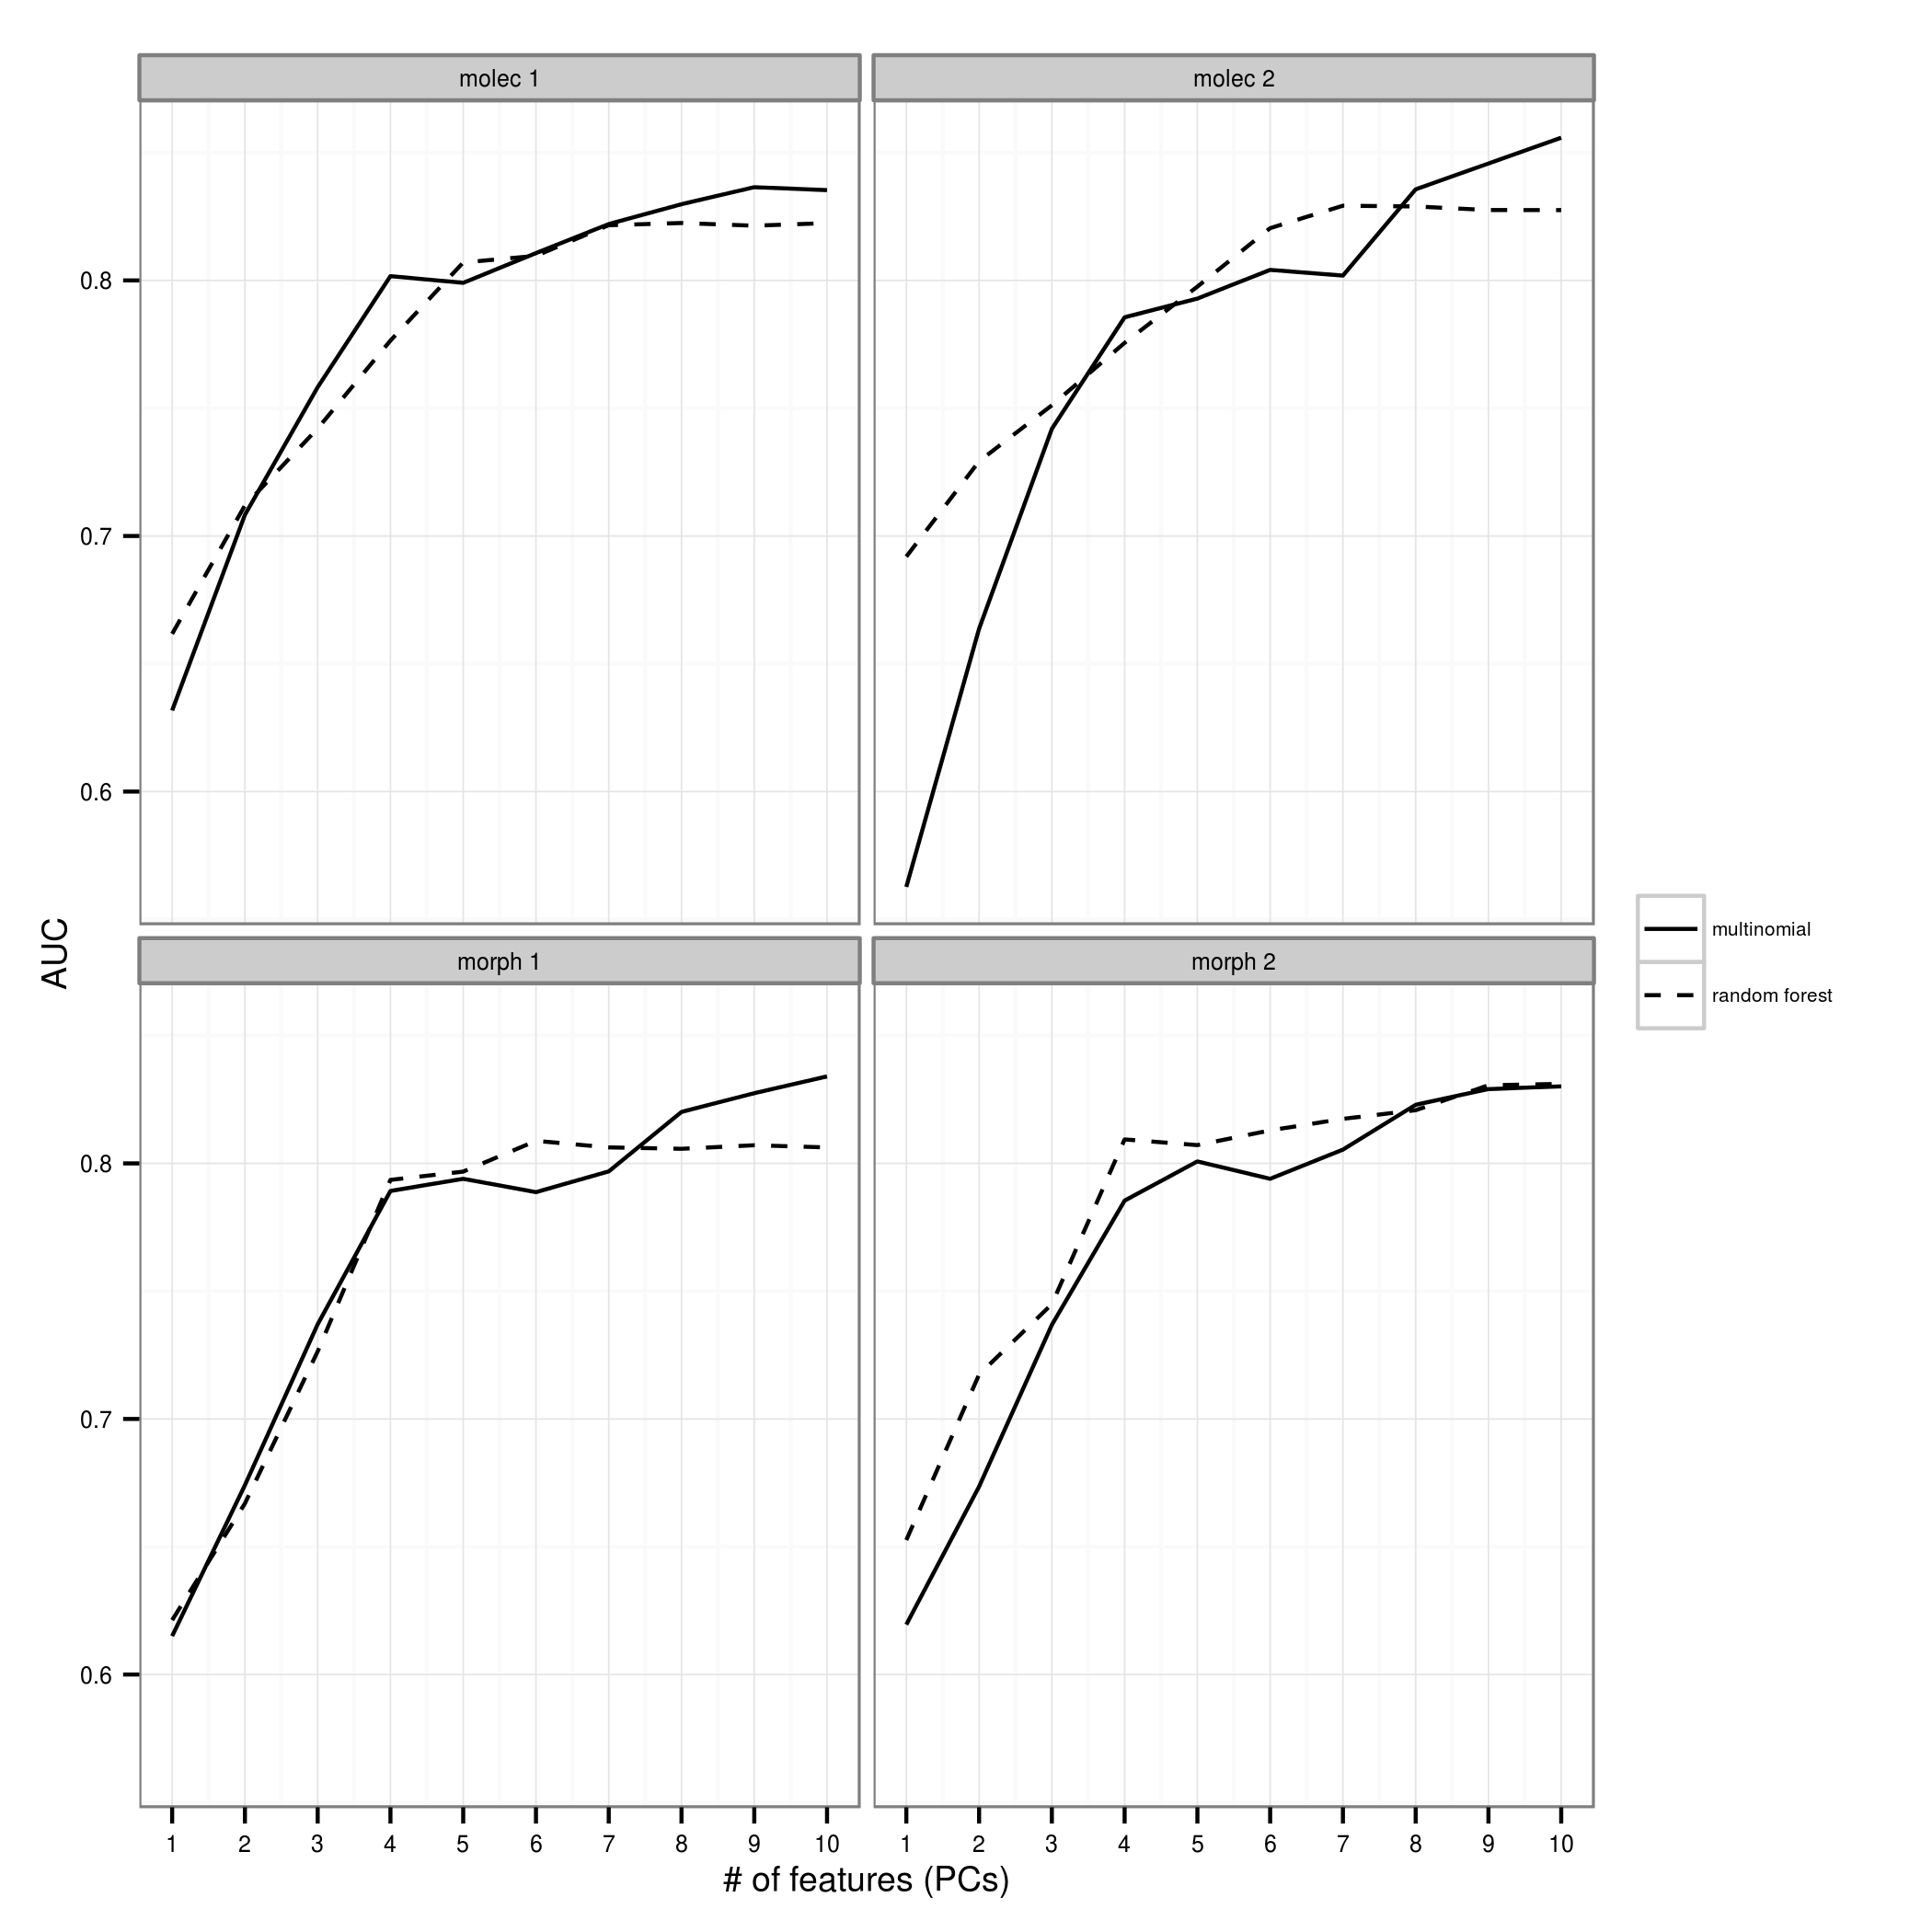
\includegraphics[width = \textwidth]{figure/roc_sel}
  \caption{Effect of increasing the number of PCs as features, or predictors, of classification of plastra for all four classification schemes. As the number of PCs increase, AUC ROC increases until eventually leveling off. Both multinomial logisitic regression and random forest models are illustrated here, though AUC ROC based model selection was only performed for random forest models.}
  \label{fig:roc}
\end{figure}

% table
%   AICc model selection
%   SUPPLEMENT?

%   maps
%     facet: training, multinomial, rf
Results of the bootstrap resamples of the AUC ROC of the generalization of the selected multinomial logistic regression and random forest models demonstrates that one of the molecular classification hypotheses based on \citet{Spinks2005} and \citet{Spinks2010} appears to be the best classification scheme (Fig. \ref{fig:gen_res}). The distribution of bootstrapped AUC ROC for the molecular hypothesis is significantly different MANN-WHITNEY U TEST and greater than all of the other classification scheme. What is remarkable is that the best classification hypothesis is identical based on both the multinomial logistic regression and random forest models.

\begin{figure}[ht]
  \centering
  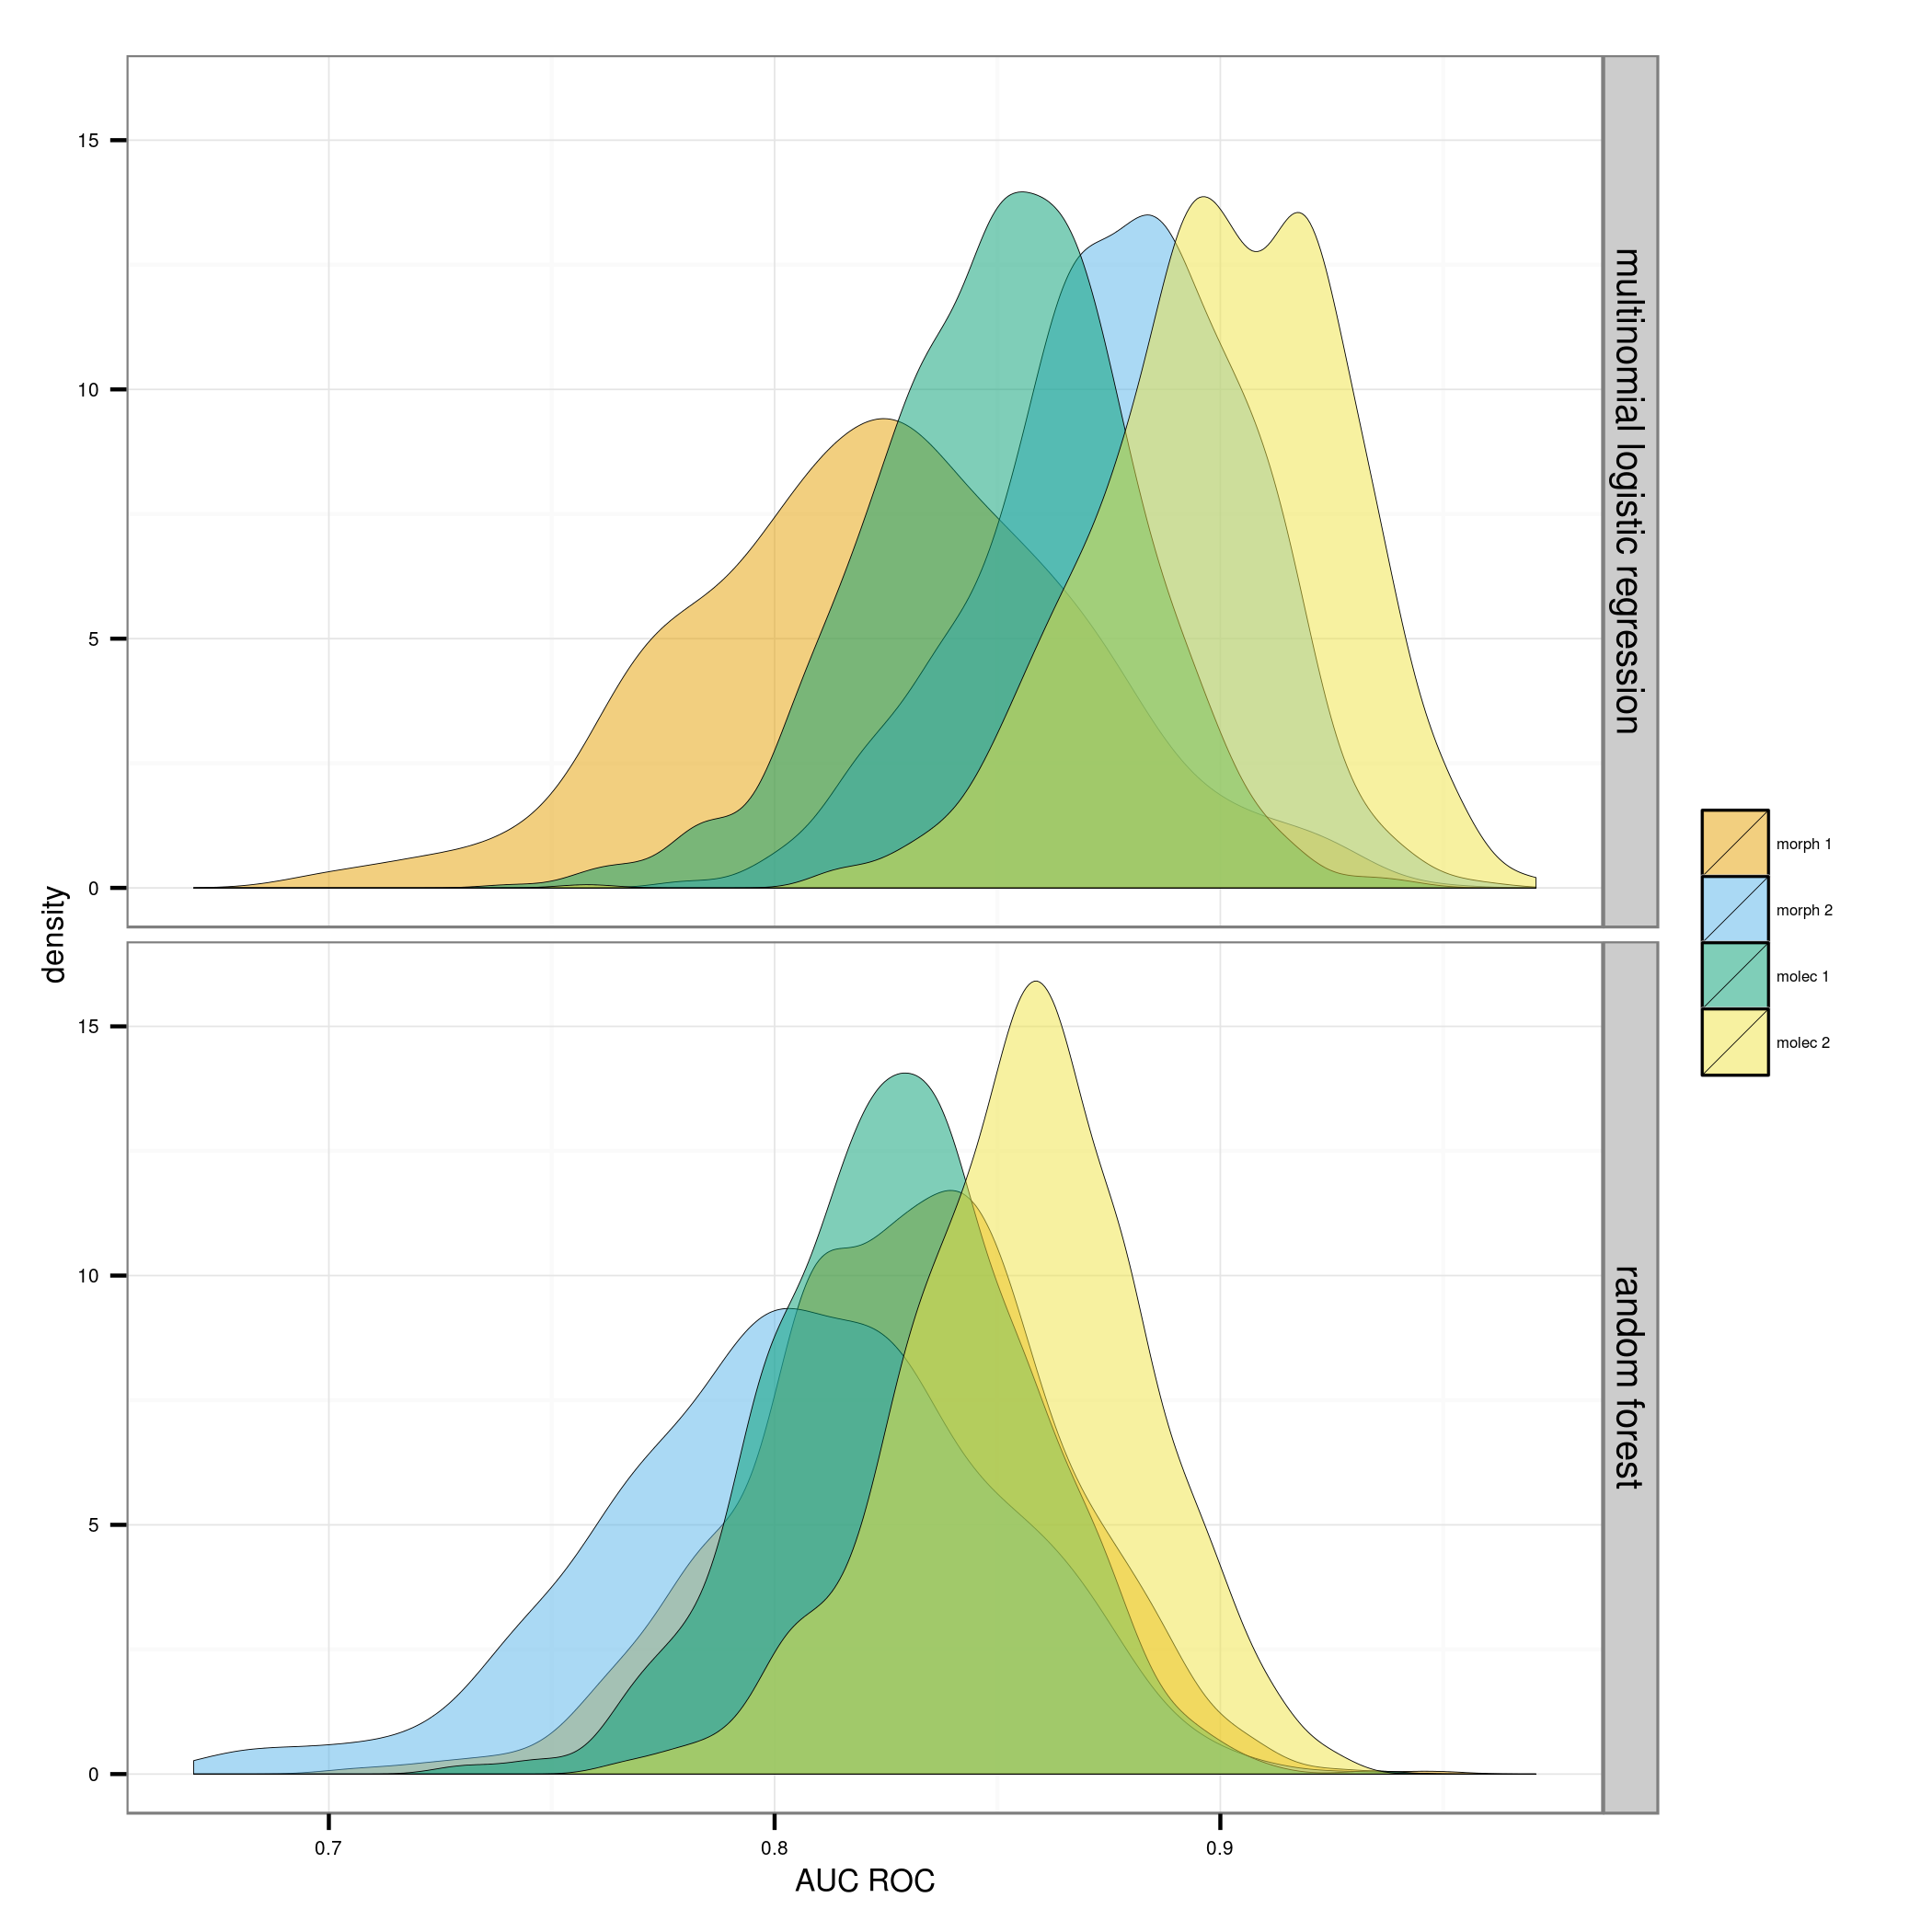
\includegraphics[width = \textwidth]{figure/gen_res}
  \caption{Density estimates of AUC ROC values of predictions of the testing dataset of plastra from 1000 bootstrap resamples. The top facet corresponds to values using the optimal multinomial logistic regression model, as chosen by minimum AICc value. The bottom facet corresponds to the values using the optimal random forest model, as chosen by maximum AUC ROC value.}
  \label{fig:gen_res}
\end{figure}

When the classification results of the training set for the optimal classification scheme are compared with the references classes, the higher AUC ROC value of the best multinomial logistic regression model becomes apparent as the classifications are in general much more similar to the reference (Fig. \ref{fig:gen_map}). The best random forest model misclassified many of the observations as the northern clade. This trend is observable but not as exaggerated in the results of the classifications of the multinomial logistic regression model.

\begin{figure}[ht]
  \centering
  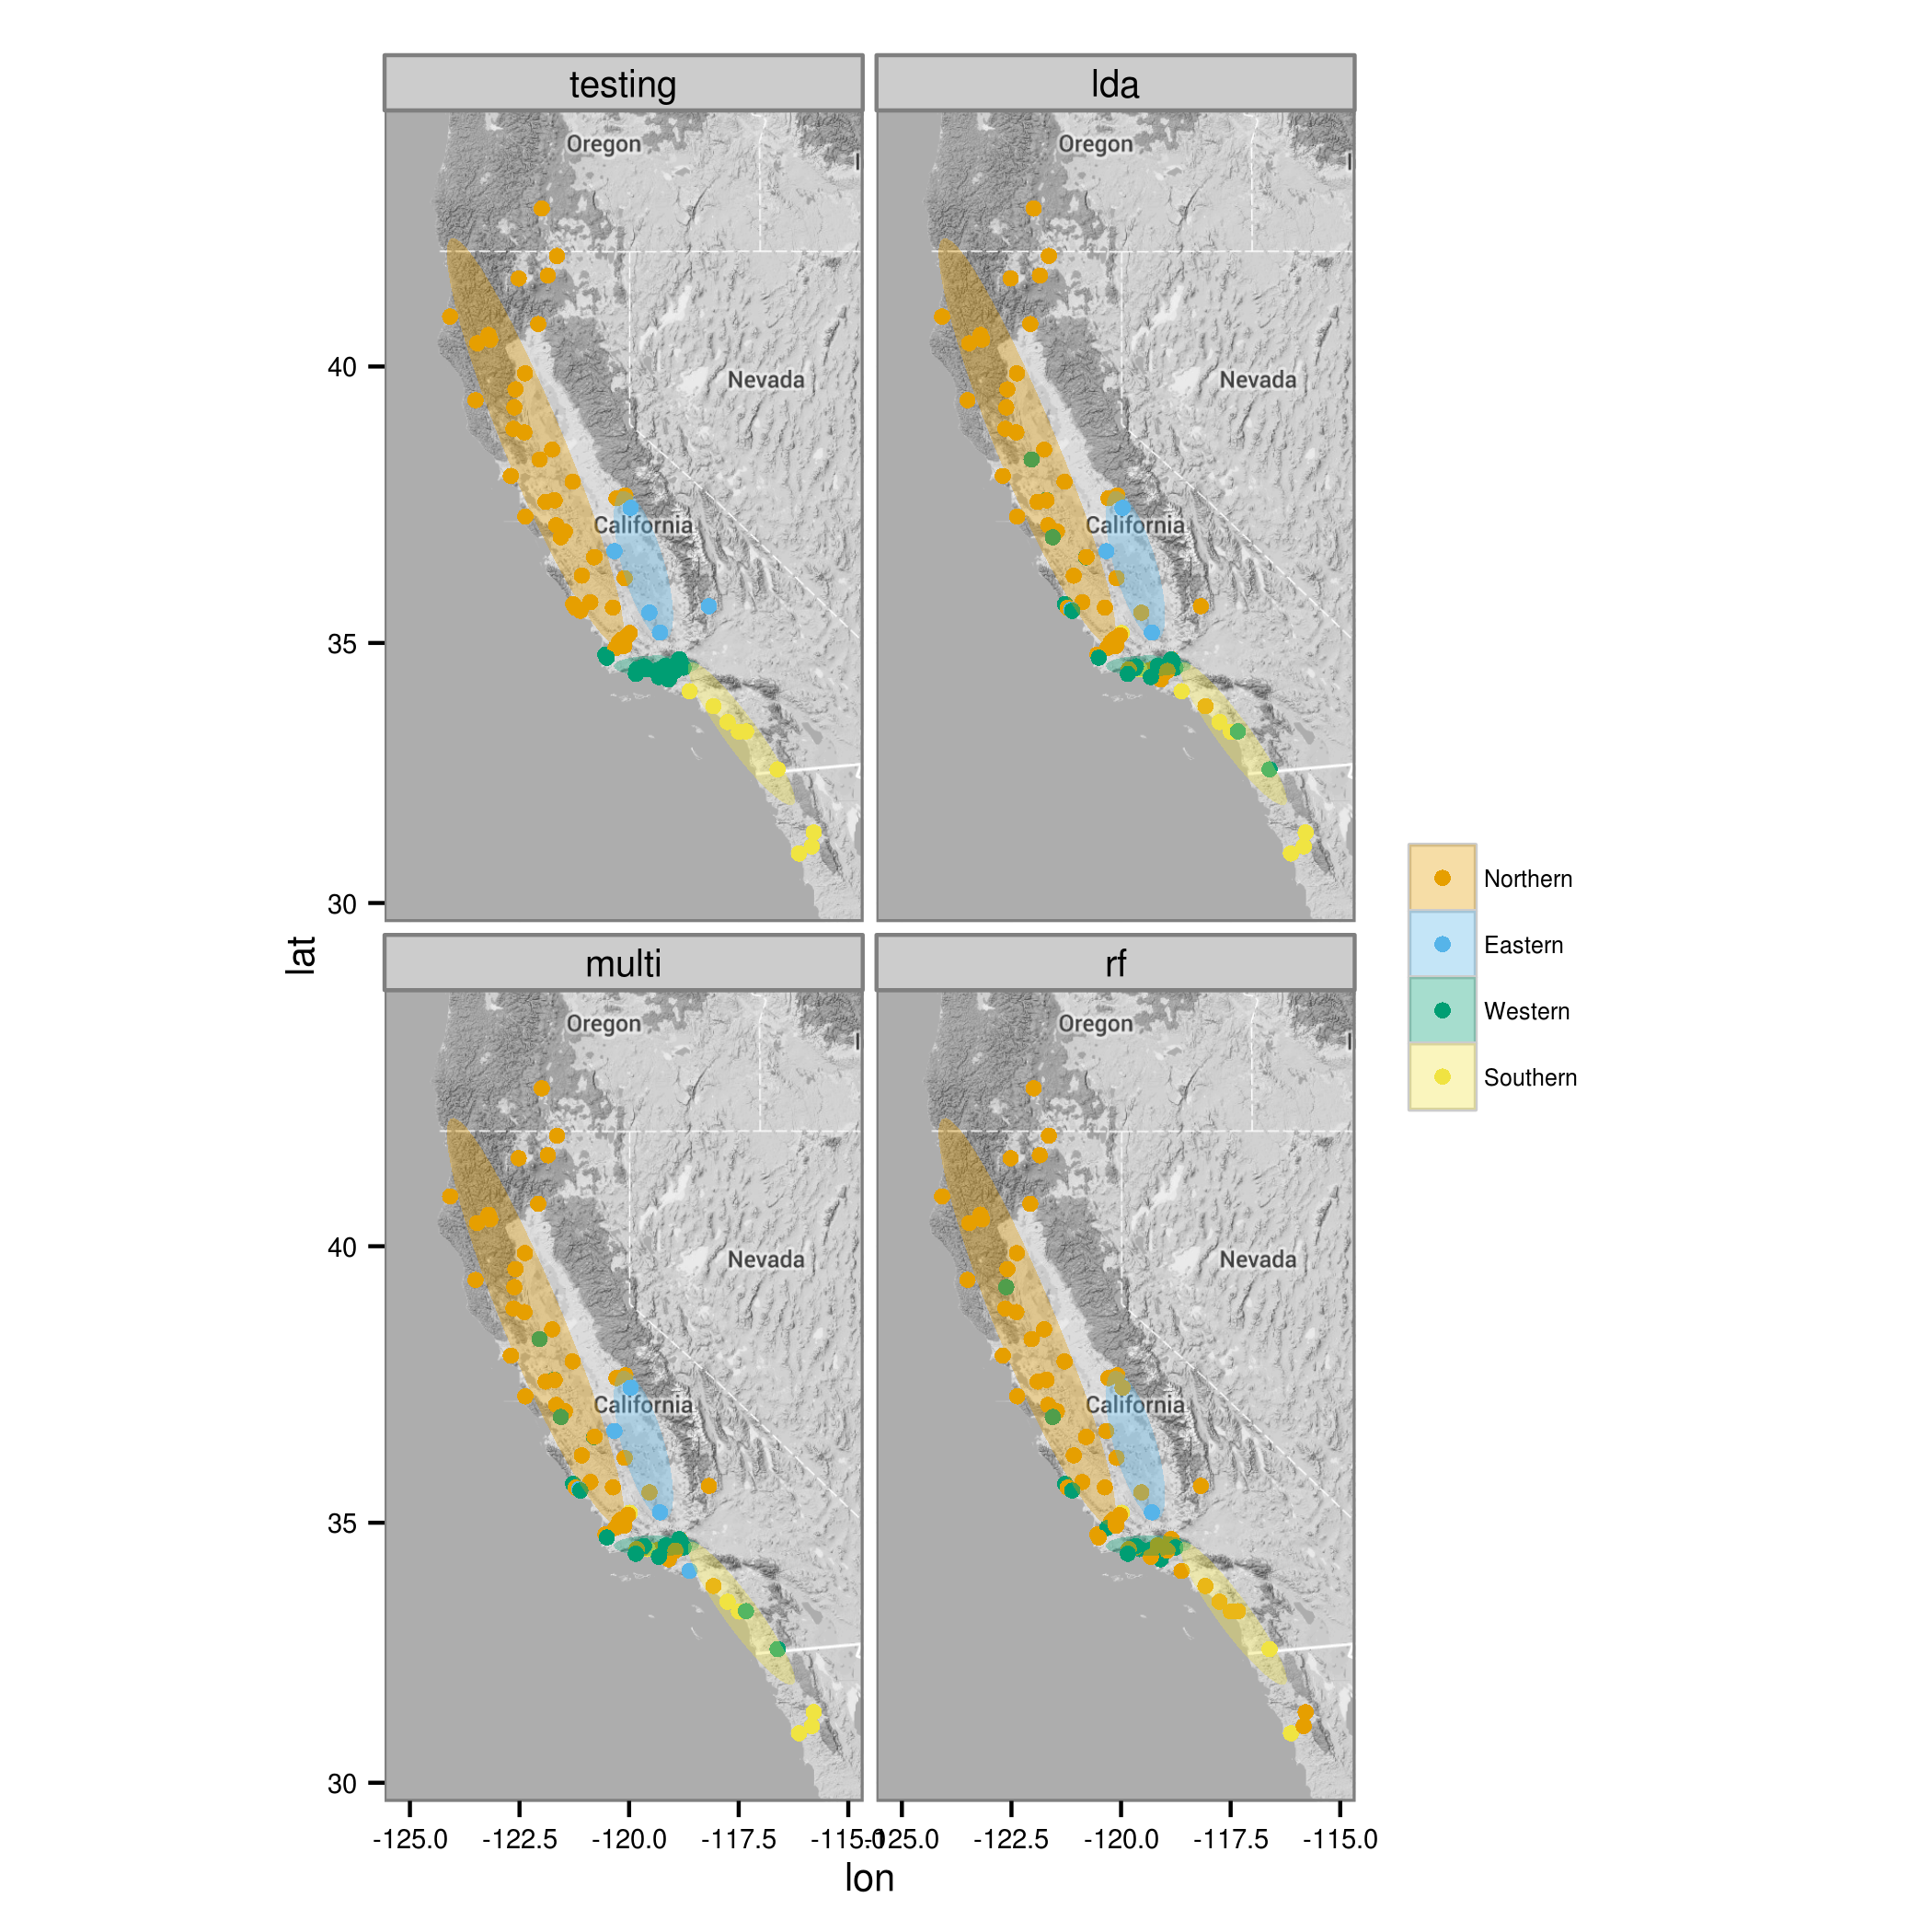
\includegraphics[width = \textwidth]{figure/gen_map}
  \caption{Comparison between reference classification of testing data set and the estimated classifications based on the selected multinomial logistic regression and random forest models, from left to right respectively. Classification corresponds to the four classes as suggested by the hypothesis of \citet{Spinks2005} and \citet{Spinks2010}.}
  \label{fig:gen_map}
\end{figure}

This pattern of misclassification may be caused by the differences in mean shape between each of the different classes (Fig. \ref{fig:mean_shape}). The mean shape of the northern clade is the most similar to the mean shape of the entire dataset (Fig. ), which may mean that specimens that are closer to the mean shape will be systematically misclassified as the northern clade.

% mean shapes of all the classes
\begin{figure}[ht]
  \centering
  \begin{subfigure}[b]{0.4\textwidth}
    \centering
    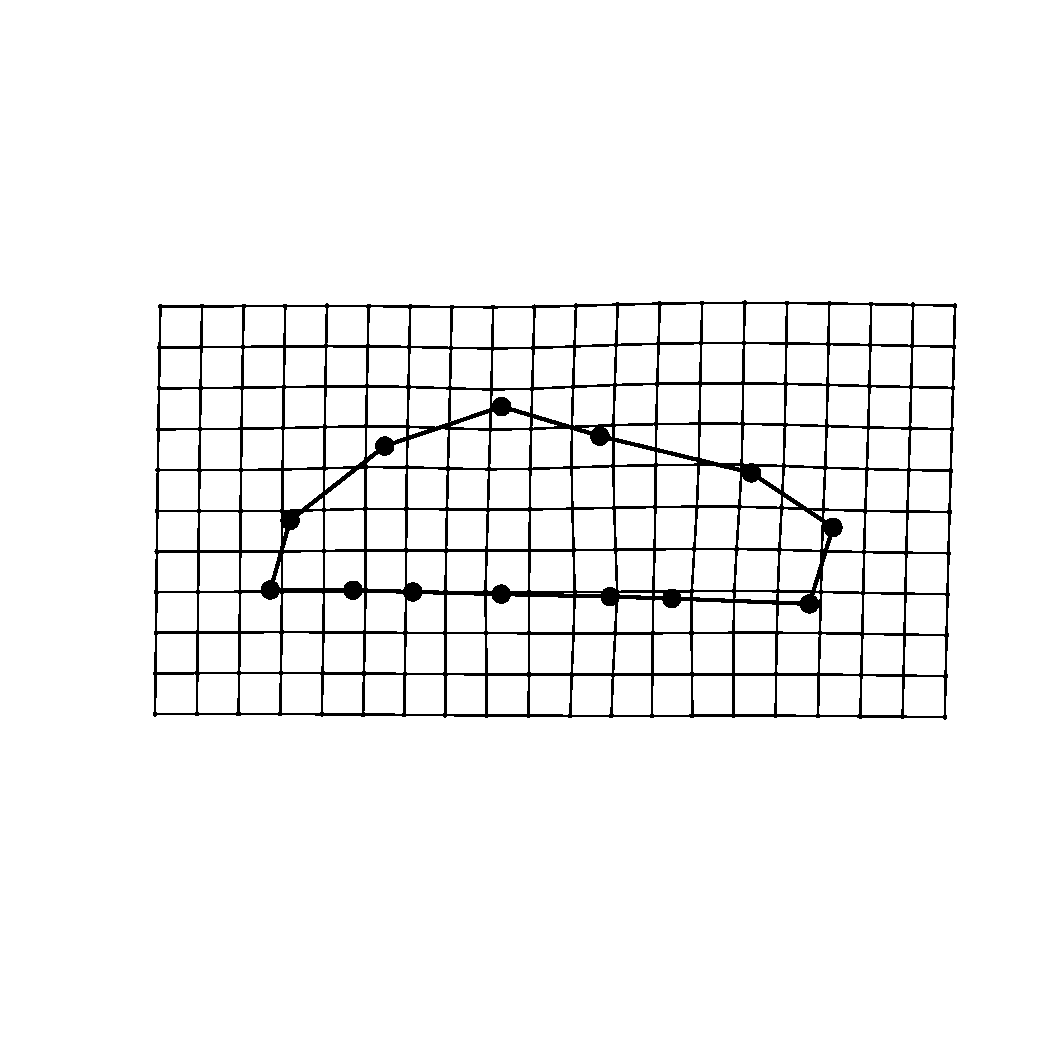
\includegraphics[width = \textwidth]{figure/mshape_1}
    \label{fig:mean_shape1}
  \end{subfigure}
  \begin{subfigure}[b]{0.4\textwidth}
    \centering
    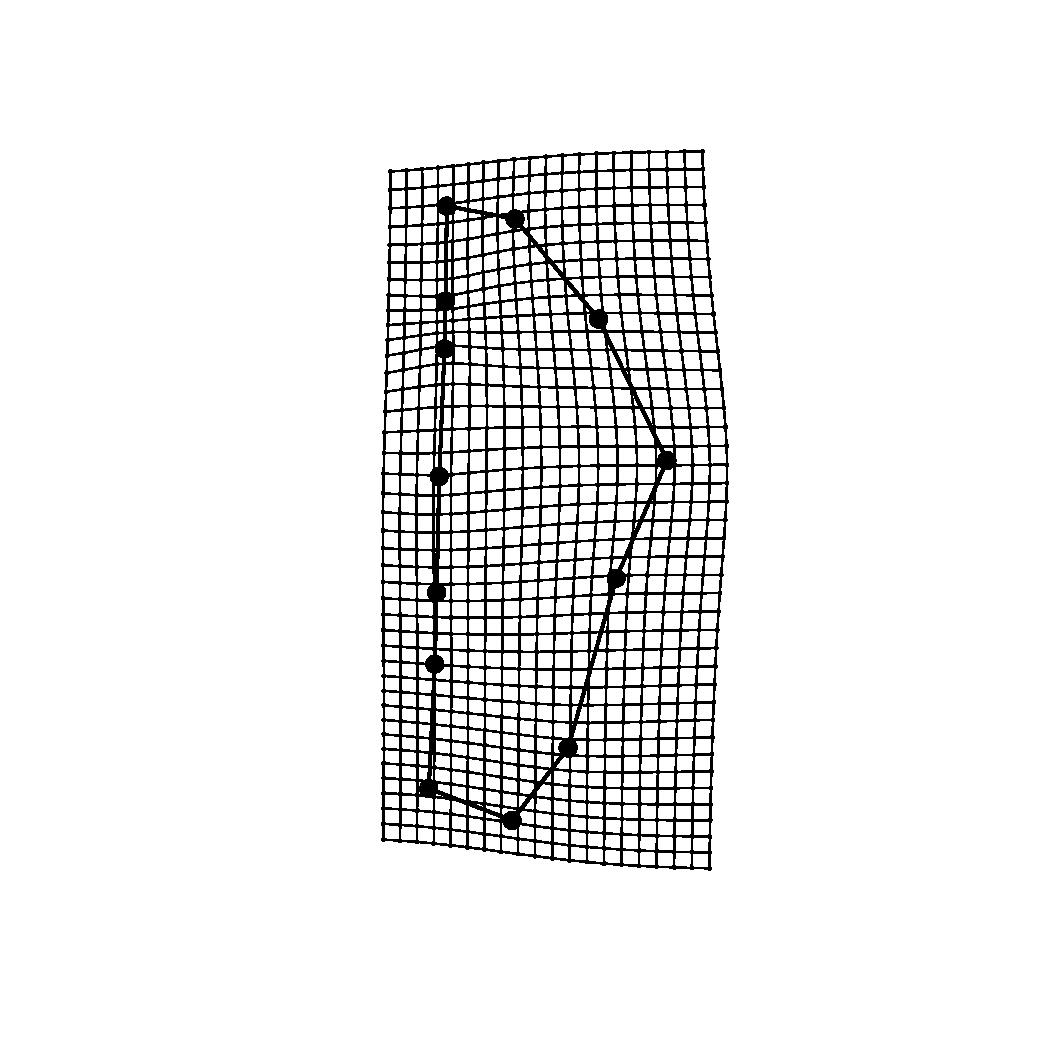
\includegraphics[width = \textwidth]{figure/mshape_2}
    \label{fig:mean_shape2}
  \end{subfigure}
  % new line. might want to make these closer together

  \begin{subfigure}[b]{0.4\textwidth}
    \centering
    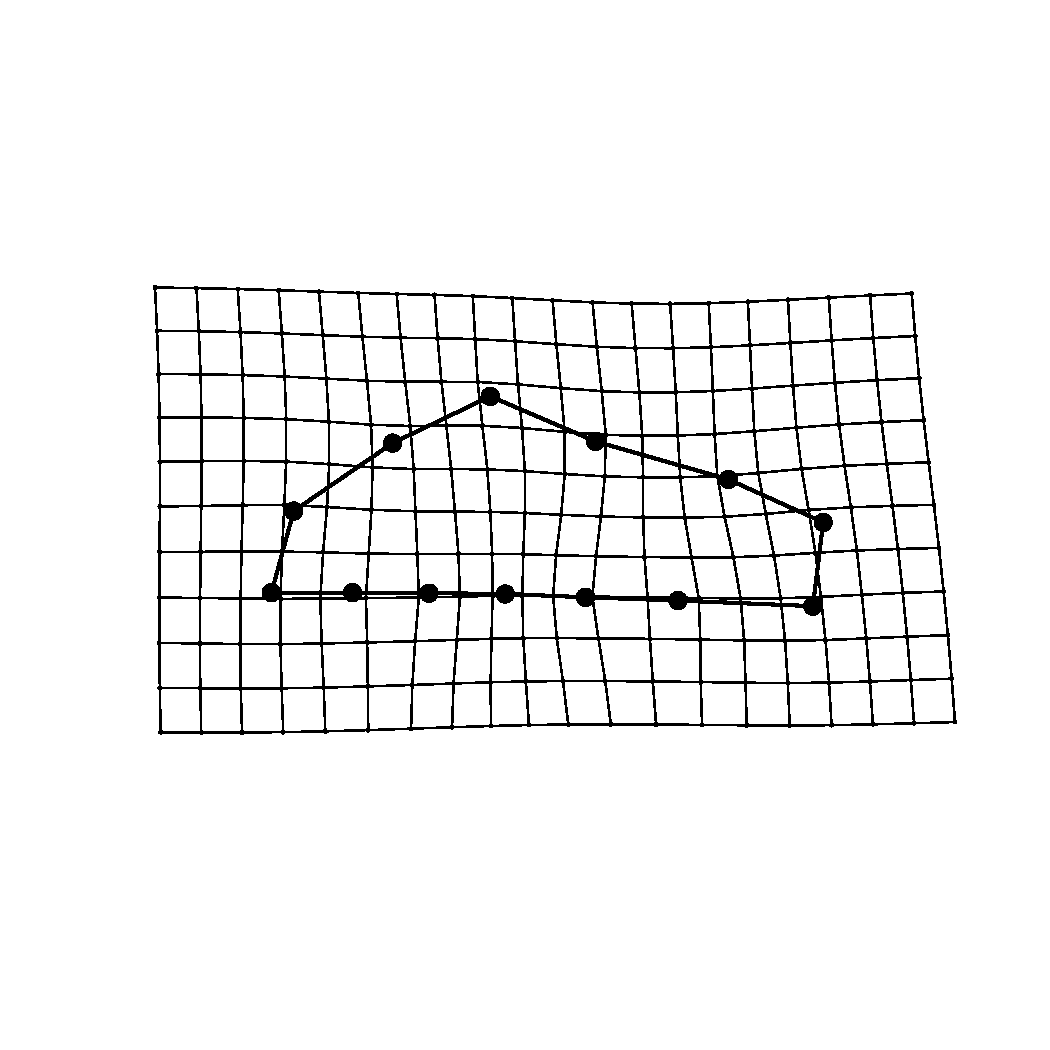
\includegraphics[width = \textwidth]{figure/mshape_3}
    \label{fig:mean_shape3}
  \end{subfigure}
  \begin{subfigure}[b]{0.4\textwidth}
    \centering
    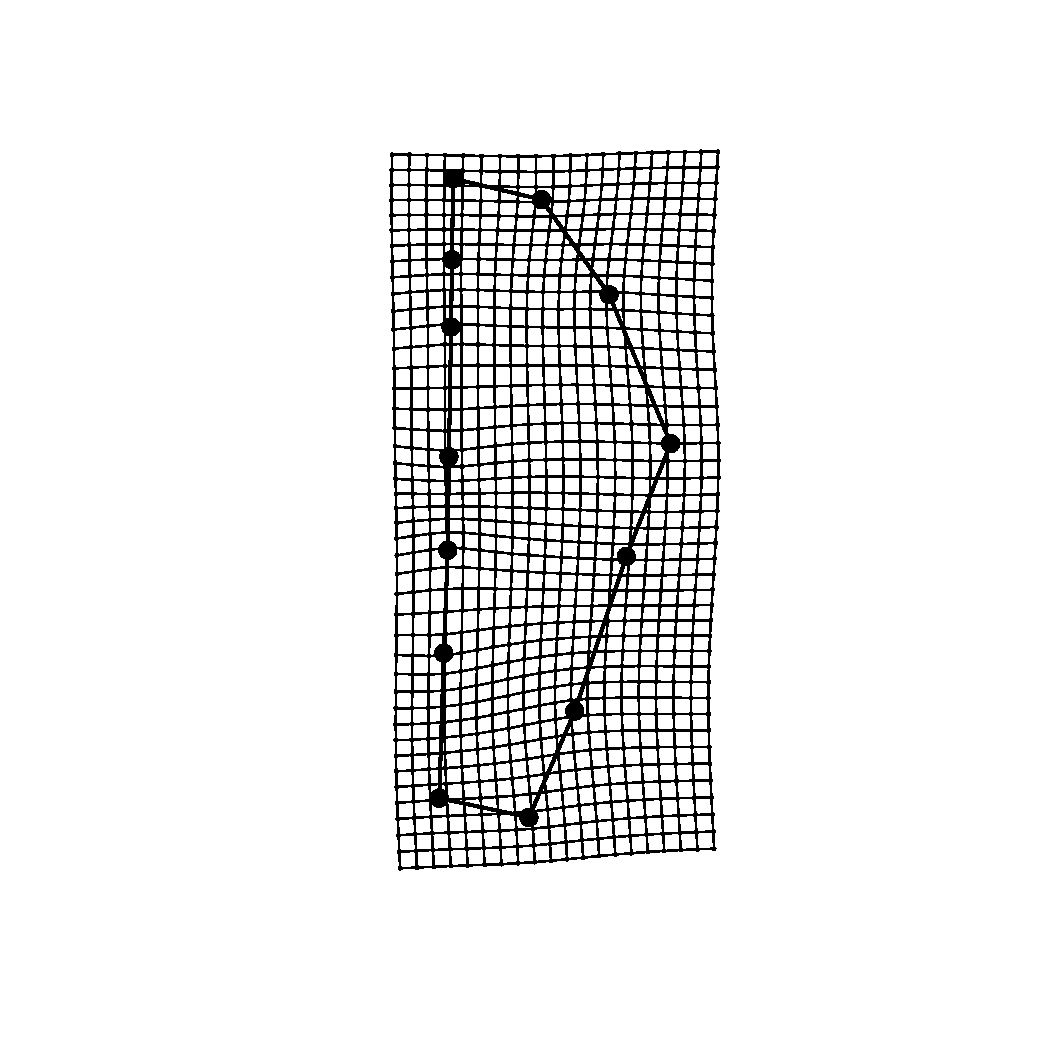
\includegraphics[width = \textwidth]{figure/mshape_4}
    \label{fig:mean_shape4}
  \end{subfigure}
  \caption{<+caption text+>}
  \label{fig:mean_shape}
\end{figure}

% variation along the most important axes
The results of training the random forest model also include the variable importance for best separating the different classes. Recursive feature selection of the best random forest model of the chosen classification scheme indicated that after 7 PCs were included as features, AUC ROC would not increase. Of these 7 features, three are illustrated here (Fig. \ref{fig:imp_pc}) the first two of which are most important SUPPLEMENT WITH VARIABLE IMPORTANCE INFORMATION?. 

\begin{figure}[ht]
  \centering
  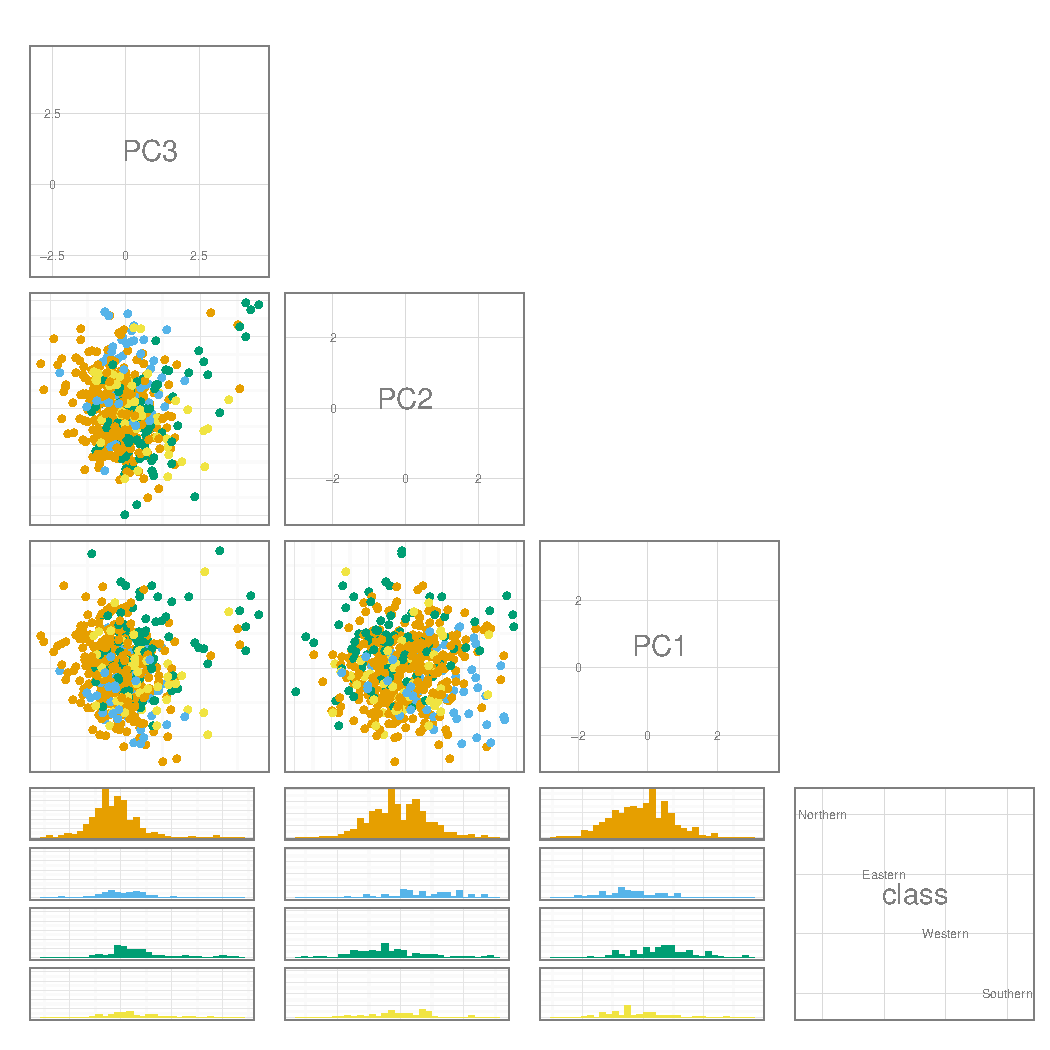
\includegraphics[width = \textwidth]{figure/pca_imp}
  \caption{Pairs plot of the first three most important variables of the optimal random forest model of turtle plastral shape. The variables descend in importance from the upper left to the lower right. The observations are colored as in Figures \ref{fig:gen_res} and \ref{fig:gen_map}.  The bottom row are histograms of classification occurrences along the PCs.}
  \label{fig:imp_pc}
\end{figure}
% need to add in variance percentages on the different axes.

The first two most important features, according to the random forest model, describe different aspects of variation (Fig. \ref{fig:imp_var}). The third PC, or first most important PC, describes variation in the relative position of landmarks on anterior and posterior portions of the plastron. The eighth PC, or second most important PC, mostly describes variation in landmarks along the midline of the plastron. The major variation along these axes correspond well to the differences between the class means and the mean plastron shape (Fig. \ref{fig:mean_shape}) where major class differences seems restricted to the relative ballooning or shrinking of the anterior and posterior portions of the plastron together.

\begin{figure}[ht]
  \centering
  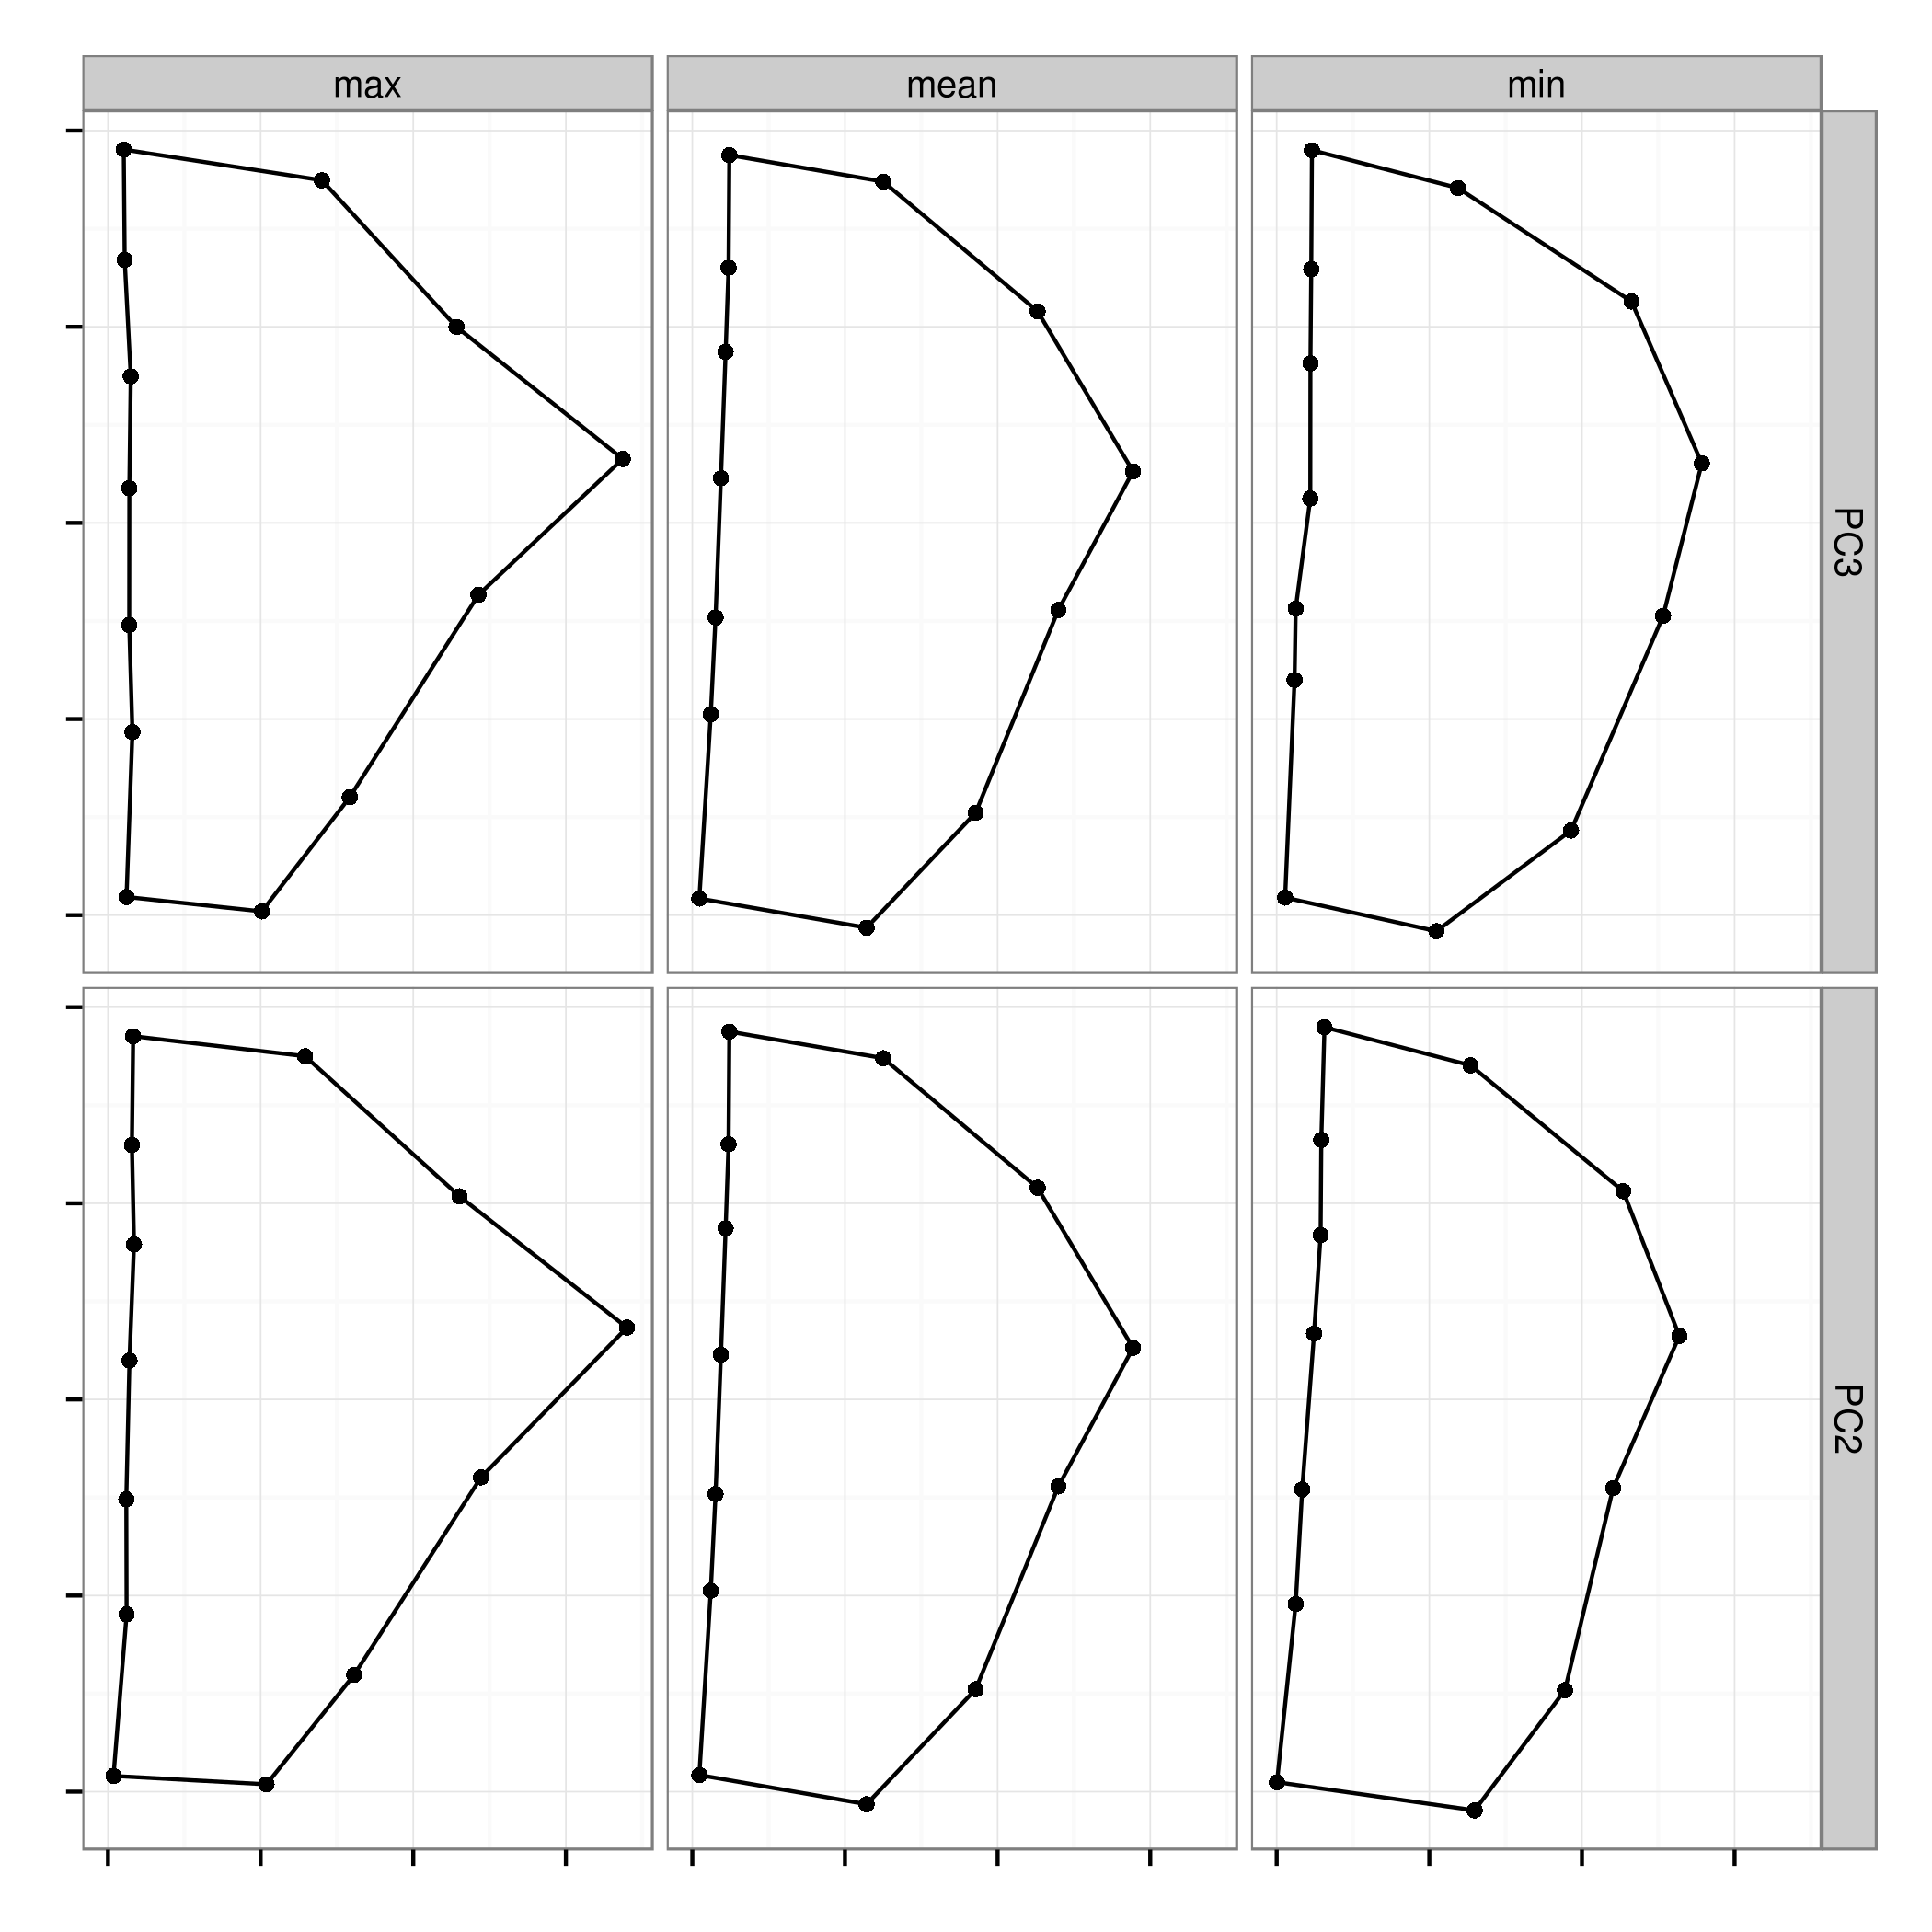
\includegraphics[width = \textwidth]{figure/imp_var}
  \caption{Landmark variation along the two most important features (PCs) based on the final random forest model. The first row corresponds to the third PC and the second corresponds to eighth PC. Landmark configurations are minimum observed on that PC, mean shape, and maximum observed on that PC.}
  \label{fig:imp_var}
\end{figure}

\section{Discussion}
% discussion of results
%   remarkable concordance in the supervised learning methods
The results of this study provide support for the mitochrondial based hypothesis of classification of \textit{E. marmorata} \citep{Spinks2005,Spinks2010}. This is contrary to the original classification of \textit{E. marmorata} \citep{Seeliger1945} and lends credence to the idea that at least some aspect of cryptic diversity is a product either sample size, methodology, or both.
%   what does this mean about cryptic diversity?
%   unsupervised learning shortcomings

The lack of coherent geographical subclass assignment from PAM based clustering (Fig. \ref{fig:gap}) as well as the large number of features necessary before plateau in AUC ROC for all models (Fig. \ref{fig:roc}) can be taken as indicators that the variation between subclasses is extremely fine grained. This is also exemplified by the differences in mean class shape for the final chosen classification scheme (Fig. \ref{fig:imp_var}).

% methodological concerns
%   compromise in the supervised learning models
%     fair because as much variation as ``necessary'' is used
%   unsupervised learning
%     model based clustering
%     nonparametric bayesian approach
%     anything about semisupervised clustering? probably not
Ultimately, it would be optimal to not require such explicit classification hypotheses, especially when concerned about possible cryptic variation in extinct taxa. The method employed in this study, PAM, is rather simple and not model based. Comparison is facilitated by comparison of a summary statistic and bootstrap confidence intervals. A more useful and future avenue would be employing various model based clustering approaches CITATIONS. In this manner, a series of candidate models can be compared via model comparison methods, such as AIC or Bayes factors CITATION, in order to asses the best clustering solution. Of particular note are nonparametric Bayesian approaches to model based clustering CITATIONS. This approach uses a class of flexible priors to allow for the most optimal clustering solution to be decided from the data. Currently, there exists a nonparametric Bayesian clustering method and further development of this approach may prove extremely fruitful for better deliminating taxa solely from morphology.

% future directions
%   conservation utility
%   fossil diversity
%     current approach favors having an extremely explicit classification hypothesis
%     as indicated about, nonparametric bayes and other model based clustering can help

% closing statements
In this study we have demonstrated that given a large sample size and appropriate methodology, it is possible to determine which of multiple hypothesized classification schemes best explain variation in a taxon. The plastral variation of \textit{E. marmorata} is most consistent with the mitochondrial based hypothesis of \citet{Spinks2005} and \citet{Spinks2010} and not with the original morphology based hypothesis of \citet{Seeliger1945}. We have also demonstrated the utility of various machine learning approaches to understanding variation in morphometric data. Specifically, better understanding odds misclassification and identifying which is the most important for deliminating different classes.

\section*{Acknowledgements}
PDS would like to thank David Bapst, Michael Foote, Benjamin Frable, and Dallas Krentzel for useful discussion which enhanced the quality of this study.

\bibliographystyle{sysbio}
\bibliography{turtle,packages}

\end{document}
